% ─────────────────────────────────────────────────────────────────────────────
% This chapter provides detailed specifications of the system under development.

\section{Introduction}

\subsection{Purpose}
This document defines the requirements for the \textbf{BookForMe} platform.  The
system's core purpose is to simplify booking of informal, local services (sports
courts, salons, gaming zones, etc.) in Karachi.  The conversational booking assistant
is embedded directly inside the mobile application.  It collects user requirements
via natural language, performs clarifying questions, and books directly from the
application's internal database when matching slots exist.

When the user requests slots that are not present in the application's internal
database and explicitly consents to external outreach, the system triggers an
\textbf{Outreach Agent} workflow.  The Outreach Agent consults a maintained contact
list of vendor numbers, selects candidate vendors matching the user's criteria,
sends structured inquiries to those vendors, ingests their replies, and presents
collected external availability options back to the user.  Outreach-sourced vendors
are presented as informational only (including contact details and parsed
availability); the user must contact such vendors directly to complete a booking.

Additionally, all onboarded vendors can link their WhatsApp Business number to the
platform's \textbf{AI Receptionist}, which then autonomously handles booking
conversations on their behalf---checking availability, locking slots via OCC, verifying
payment via OCR, and notifying the vendor for final approval.

\subsection{Scope}
The BookForMe system comprises four primary components:

\begin{enumerate}
  \item \textbf{In-App Conversational Booking Interface:} Natural-language chatbot
        embedded in the React Native mobile app that handles synchronous user
        interaction, clarifications, and direct bookings from the internal database.
  \item \textbf{Vendor Dashboard:} Vendor-facing interface for onboarding, profile
        management, calendar viewing, booking approvals, and linking WhatsApp Business
        API or Google Sheets integrations.
  \item \textbf{AI Receptionist (WhatsApp Agent):} Autonomous agent deployed on the
        vendor's WhatsApp Business number.  Handles bilingual inbound booking requests
        end-to-end, from NLU to payment verification to vendor notification.
  \item \textbf{Outreach Agent:} Upon user consent, dispatches structured inquiries
        to external vendor contacts, parses responses into canonical availability
        format, and returns informational options to the user.
  \item \textbf{Core Backend Services:} Firestore database, NLU/LLM interfaces,
        WhatsApp Business API messaging gateway, OCR service, and Firebase
        Authentication.
\end{enumerate}

% ─────────────────────────────────────────────────────────────────────────────
\section{Functional Requirements}

This section describes each function/feature provided by our system.  These
functions are logically grouped into modules based on purpose and users.

\begin{outline}

  \1 \textbf{Module: Customer / User (Booking \& Discovery)}
  \2 \texttt{FR-CUST-01}: The system shall allow users to browse and search registered
       vendors by service category (e.g., Futsal, Salon, Gaming Zone) and location area.
  \2 \texttt{FR-CUST-02}: The system shall provide filtering options (price range,
       rating, amenities such as parking, WiFi, AC courts).
  \2 \texttt{FR-CUST-03}: The system shall display vendor profiles including name,
       description, location, services offered, pricing, reviews, and ratings.
  \2 \texttt{FR-CUST-04}: The system shall display any discounts or promotions offered
       by a vendor.
  \2 \texttt{FR-CUST-05}: The system shall present users with a calendar interface
       showing real-time available and booked time slots.
  \2 \texttt{FR-CUST-06}: The system shall allow users to select an available time slot,
       add it to a cart, review the booking summary, and confirm checkout.
  \2 \texttt{FR-CUST-07}: The system shall allow users to upload a payment screenshot
       after booking confirmation.
  \2 \texttt{FR-CUST-08}: The system shall confirm successful bookings to the user via
       the app interface, notifications page, and optionally a WhatsApp confirmation.

  \1 \textbf{Module: Customer / User (Interaction \& Feedback)}
  \2 \texttt{FR-CUST-09}: The system shall allow users to leave a star rating and text
       review for a vendor after a completed booking.
  \2 \texttt{FR-CUST-10}: The system shall provide an on-app AI chatbot capable of
       parsing natural-language queries (English / Roman Urdu) and performing
       cross-category filtered searches against the platform's internal database.
  \2 \texttt{FR-CUST-11}: The system shall provide a notifications page for booking
       status updates, friend requests, and direct messages.
  \2 \texttt{FR-CUST-12}: The system shall allow users to consent to external outreach
       when no internal matches satisfy their request; the system shall then trigger the
       Outreach Agent (\texttt{FR-OUT-01} -- \texttt{FR-OUT-10}).

  \1 \textbf{Module: Customer / User (Social \& Community)}
  \2 \texttt{FR-SOC-01}: The system shall provide user registration and login
       (email/password and Google OAuth).
  \2 \texttt{FR-SOC-02}: The system shall allow users to create and manage a public
       profile (username, avatar, match history, Elo rating).
  \2 \texttt{FR-SOC-03}: The system shall allow users to search for other users on
       the platform.
  \2 \texttt{FR-SOC-04}: The system shall provide a friend system: send, accept,
       and decline friend requests.
  \2 \texttt{FR-SOC-05}: The system shall allow users to send and receive private
       direct messages with users on their friends list.
  \2 \texttt{FR-SOC-06}: The system shall provide a community forum where users can
       create, view, like, and comment on public posts.
  \2 \texttt{FR-SOC-07}: The system shall provide a mechanism for users to report
       other users or posts for moderation.

  \1 \textbf{Module: Customer / User (Matchmaking \& Ranking)}
  \2 \texttt{FR-MATCH-01}: The system shall provide a mechanism for users to queue
       for a Casual Match (no rating impact).
  \2 \texttt{FR-MATCH-02}: The system shall provide a mechanism for users to queue
       for a Ranked Match, matched by Elo rating within a configurable window
       ($\pm 200$ points, expanding with wait time).
  \2 \texttt{FR-MATCH-03}: The system shall calculate and update user Elo ratings
       based on ranked match outcomes.
  \2 \texttt{FR-MATCH-04}: The system shall display a public leaderboard of top-ranked
       players, filterable by sport.

  \1 \textbf{Module: Vendor}
  \2 \texttt{FR-VEND-01}: The system shall provide secure vendor registration, login,
       and profile management (business name, category, location, services, pricing,
       operating hours, media).
  \2 \texttt{FR-VEND-02}: Vendors shall be able to link their WhatsApp Business API
       account to activate the AI Receptionist for inbound WhatsApp bookings.
  \2 \texttt{FR-VEND-03}: Vendors shall be able to link a Google Sheets document for
       automatic schedule synchronisation.
  \2 \texttt{FR-VEND-04}: Vendors shall be able to view a consolidated calendar
       showing all bookings from all channels (web app, WhatsApp, Sheets) in one place.
  \2 \texttt{FR-VEND-05}: The system shall provide an interface for vendors to
       manually add, update, search, export, and delete bookings.
  \2 \texttt{FR-VEND-06}: The system shall provide a Pending Approvals interface
       where vendors can review a booking (customer, service, time, payment screenshot)
       and approve or reject it.
  \2 \texttt{FR-VEND-07}: Vendors shall be able to view basic analytics: total
       bookings today, monthly revenue, occupancy rate, and recent activity.

  \1 \textbf{Module: AI Receptionist (WhatsApp Agent)}
  \2 \texttt{FR-AGENT-01}: The system shall receive inbound WhatsApp messages via a
       configured Meta/Twilio webhook.
  \2 \texttt{FR-AGENT-02}: The system shall send outbound WhatsApp messages
       (replies, confirmations, rejection notices) via the WhatsApp Business API.
  \2 \texttt{FR-AGENT-03}: The system shall process inbound messages (English /
       Roman Urdu) to extract intent and slot entities (service, date, time,
       duration, budget, location).
  \2 \texttt{FR-AGENT-04}: The system shall maintain full conversational context
       (dialogue state) for ongoing WhatsApp interactions, persisted in Firestore
       across arbitrary delays.
  \2 \texttt{FR-AGENT-05}: Based on NLU output and availability, the system shall
       determine and execute appropriate actions (confirm availability, offer
       alternatives, create HOLD booking, request payment, process payment, notify
       vendor).
  \2 \texttt{FR-AGENT-06}: The system shall implement Optimistic Concurrency Control
       via Firestore transactions to prevent conflicting bookings for the same time
       slot across all channels simultaneously.
  \2 \texttt{FR-AGENT-07}: The system shall parse linked Google Sheets to identify
       manually entered bookings and synchronise them to the central Firestore
       database.
  \2 \texttt{FR-AGENT-08}: After verbal confirmation of a booking, the system shall
       request the user to submit a payment screenshot (advance payment) and set the
       booking status to \texttt{HOLD} with a 10-minute expiry.
  \2 \texttt{FR-AGENT-09}: The system shall process the uploaded payment screenshot
       using OCR to extract the transferred amount.  If the amount does not match
       the required advance payment, the system shall automatically reject the
       screenshot and request a corrected one without notifying the vendor.
  \2 \texttt{FR-AGENT-10}: Upon successful OCR verification, the system shall update
       the booking to \texttt{PENDING\_APPROVAL}, attach the screenshot to the
       booking record, and notify the vendor on the Vendor Dashboard.
  \2 \texttt{FR-AGENT-11}: Upon vendor approval, the system shall update booking
       status to \texttt{CONFIRMED} and send a confirmation message with a ticket ID
       to the user on WhatsApp.

  \1 \textbf{Module: Outreach (Informational-only external discovery)}
  \2 \texttt{FR-OUT-01}: When user consents, create an Outreach Job encapsulating
       the user's criteria and preferences.
  \2 \texttt{FR-OUT-02}: Select and rank vendor contacts from the maintained contact
       list based on relevance (location, service type, historical responsiveness).
  \2 \texttt{FR-OUT-03}: Dispatch structured outreach inquiry messages to selected
       vendor contacts via the WhatsApp / SMS messaging gateway using pre-defined
       templates.
  \2 \texttt{FR-OUT-04}: Receive vendor replies and normalise them into canonical
       availability records (start time, end time, price, hold-ability if stated).
  \2 \texttt{FR-OUT-05}: Aggregate and deduplicate external availability options;
       compute parsing confidence for each.
  \2 \texttt{FR-OUT-06}: Present each external option with vendor name, phone number,
       preferred contact channel, parsed availability, confidence score, and a clear
       disclaimer that these results are informational and require the user to contact
       the vendor directly.
  \2 \texttt{FR-OUT-07}: Store and enforce vendor outreach consent metadata;
       process opt-out requests promptly.
  \2 \texttt{FR-OUT-08}: Maintain an audit log of all outreach messages sent and
       responses received.
  \2 \texttt{FR-OUT-09}: Enforce messaging-provider rate limits and implement
       exponential back-off and retry for failed message delivery.
  \2 \texttt{FR-OUT-10}: Allow the user to cancel an ongoing Outreach Job at any
       time.

  \1 \textbf{Module: Stretch Goals (Future Scope)}
  \2 \texttt{FR-STRETCH-01}: The system may provide a payment gateway (JazzCash /
       EasyPaisa) replacing screenshot-based payment with programmatic confirmation.
  \2 \texttt{FR-STRETCH-02}: The AI Receptionist may be extended to transcribe and
       understand WhatsApp voice notes via Whisper ASR.
  \2 \texttt{FR-STRETCH-03}: The system may implement a recommendation algorithm
       (collaborative filtering, link prediction) to suggest vendors based on booking
       history and social graph.
  \2 \texttt{FR-STRETCH-04}: The system may extend to voice-call booking via Twilio
       Voice with Google/Azure speech-to-text and text-to-speech.

\end{outline}

\subsection{Use Case Interaction (Textual Representation)}

\textbf{Core interactions:}
\begin{itemize}
  \item \textbf{App Customer} uses the \textit{Mobile Application} to:
    \begin{itemize}
      \item Register, log in, and manage a profile.
      \item Search and filter vendors; view availability calendars.
      \item Select a slot, confirm booking, upload payment proof, and receive confirmation.
      \item Use the embedded AI chatbot for natural-language slot discovery.
      \item Consent to Outreach Agent when no internal match is found.
      \item Join match lobbies; post to forums; message friends; view leaderboard.
    \end{itemize}
  \item \textbf{WhatsApp Customer} uses the \textit{AI Receptionist} to:
    \begin{itemize}
      \item Send a natural-language booking request (English or Roman Urdu).
      \item Answer clarifying questions from the agent.
      \item Receive slot options and confirm a choice.
      \item Upload a payment screenshot for OCR verification.
      \item Receive a booking confirmation ticket.
    \end{itemize}
  \item \textbf{Vendor} uses the \textit{Vendor Dashboard} to:
    \begin{itemize}
      \item Register, manage business profile, and add services/slots.
      \item Link WhatsApp Business API to activate the AI Receptionist.
      \item Link Google Sheets for schedule synchronisation.
      \item View consolidated booking calendar and approve/reject pending bookings.
      \item View revenue and occupancy analytics.
    \end{itemize}
\end{itemize}

% ─────────────────────────────────────────────────────────────────────────────
\section{Non-Functional Requirements}

This section specifies the quality attributes of the system.

\subsection{Performance}
\begin{itemize}
  \item \texttt{NFR-PERF-01}: Key web/app pages (vendor search, availability calendar)
        shall load within \textbf{30 seconds} on an average stable mobile connection.
  \item \texttt{NFR-PERF-02}: The AI Agent's NLU processing for a standard WhatsApp
        message shall complete within \textbf{60 seconds}.
  \item \texttt{NFR-PERF-03}: Total time from receiving a WhatsApp availability query
        to sending the initial agent response shall not exceed \textbf{60 seconds}.
  \item \texttt{NFR-PERF-04}: The WhatsApp webhook endpoint shall be capable of
        processing at least \textbf{4 simultaneous} incoming requests without failure.
  \item \texttt{NFR-OUT-PERF-01}: Outreach job creation shall be queued within
        \textbf{2 seconds}; first batch of outreach messages shall be scheduled within
        \textbf{15 seconds} of job creation, subject to provider rate limits.
\end{itemize}

\subsection{Security and Privacy}
\begin{itemize}
  \item \texttt{NFR-SEC-01}: All user and vendor access shall be protected via
        Firebase Authentication (email/password and OAuth 2.0).
  \item \texttt{NFR-SEC-02}: All external API keys (WhatsApp, Google Sheets, Gemini)
        shall be stored as environment variables / Google Secret Manager secrets,
        never hardcoded.
  \item \texttt{NFR-SEC-03}: The WhatsApp webhook endpoint shall verify the integrity
        of all incoming requests using Meta's Verify Token.
  \item \texttt{NFR-SEC-04}: All data transmission between clients, the backend, and
        external APIs shall use HTTPS/TLS.
  \item \texttt{NFR-SEC-05}: Payment screenshots shall be stored in a private Firebase
        Storage bucket; access shall be granted only via time-limited Signed URLs to
        the specific vendor and admin.
  \item \texttt{NFR-PRIV-01}: The Outreach Agent shall only contact vendors with
        recorded consent; opt-out requests shall be processed within 24 hours.
\end{itemize}

\subsection{Reliability and Robustness}
\begin{itemize}
  \item \texttt{NFR-REL-01}: The system shall target \textbf{99.0\%} uptime during
        peak operating hours (6~PM--11~PM daily).
  \item \texttt{NFR-REL-02}: The AI Agent shall handle external API errors (NLU
        timeouts, Gemini failures) gracefully, logging errors without crashing the
        main service; a fallback rule-based handler shall respond to the user.
  \item \texttt{NFR-REL-03}: The Google Sheets synchronisation process shall be
        fault-tolerant, logging API and parsing errors without corrupting the main
        Firestore database.
  \item \texttt{NFR-OUT-RETRY-01}: Outreach message delivery failures shall be retried
        with exponential back-off (max 3 retries); all failed attempts shall be logged.
\end{itemize}

\subsection{Scalability}
\begin{itemize}
  \item \texttt{NFR-SCAL-01}: The backend application shall support horizontal scaling
        via Firebase Cloud Functions (serverless) to handle increased load.
  \item \texttt{NFR-SCAL-02}: The Firestore schema shall support baseline functionality
        for at least \textbf{100 concurrent users} without significant performance
        degradation.
  \item \texttt{NFR-SCAL-03}: The system shall support onboarding and operation for
        at least \textbf{10 vendors} simultaneously without degradation.
\end{itemize}

\subsection{Usability}
\begin{itemize}
  \item \texttt{NFR-USAB-01}: A new user shall be able to complete a booking in fewer
        than \textbf{8 primary steps} from the home screen (Search $\to$ Select
        Vendor $\to$ View Calendar $\to$ Select Slot $\to$ Confirm $\to$ Payment).
  \item \texttt{NFR-USAB-02}: All key vendor dashboard functions (calendar, approvals,
        connect APIs) shall be accessible within \textbf{6 taps} from the main
        dashboard screen.
  \item \texttt{NFR-USAB-03}: WhatsApp agent responses shall be clear, concise, and
        contextually appropriate in both English and Roman Urdu.
  \item \texttt{NFR-USAB-04}: The UI shall clearly distinguish between internally
        bookable slots (confirmed via the app) and external outreach results
        (requiring direct user contact).
\end{itemize}

\subsection{Data Integrity and Backup}
\begin{itemize}
  \item \texttt{NFR-DATA-01}: Canonicalised external availability records shall
        include a source reference and ingestion timestamp.
  \item \texttt{NFR-BACK-01}: Outreach job logs and Firestore data shall be included
        in daily automated backups.
\end{itemize}

% ─────────────────────────────────────────────────────────────────────────────
\section{SRS Part 2: System Block Diagram and Higher-Level Architecture}
\label{sec:srs-arch}

\subsection{System Block Diagram}

Figure~\ref{fig:srs-block} presents the high-level system block diagram for the
BookForMe platform.  The architecture has two primary layers: a \textbf{Frontend
Layer} and a \textbf{Backend / API Layer}.

\begin{figure}[H]
  \centering
  \IfFileExists{images/system-overview.png}{
    \includegraphics[width=0.95\textwidth]{images/system-overview.png}
  }{\IfFileExists{images/introduction/system-overview.png}{
    \includegraphics[width=0.95\textwidth]{images/introduction/system-overview.png}
  }{
    \fbox{\parbox{0.80\textwidth}{\centering\vspace{1cm}
    Missing figure asset: \texttt{images/system-overview.png}.\par
    System block diagram placeholder\vspace{1cm}}}
  }}
  \caption{System block diagram for the BookForMe platform.}
  \label{fig:srs-block}
\end{figure}

\subsection{Description of Components}

\begin{description}
  \item[User Mobile Application (Frontend)]
        Developed using \textbf{React Native (TypeScript)}, this is the native mobile
        app for customers.  It allows users to browse vendors, book services, interact
        with the embedded AI chatbot, and access all social features (profiles, chat,
        forums, matchmaking).  It communicates with the backend via RESTful JSON/HTTPS
        APIs.

  \item[Vendor Dashboard (Frontend)]
        A secure administrative interface also built with \textbf{React Native}.  It
        allows vendors to manage their business profile, view the consolidated booking
        calendar, approve or reject pending payments, and link their external WhatsApp
        Business API account and Google Sheets.

  \item[Central Backend API]
        Deployed as a \textbf{Python / FastAPI} serverless application on
        Render.com / Firebase Cloud Functions.  It is the single orchestration layer
        that: processes app API calls, routes WhatsApp webhook events to the AI Agent,
        delegates image processing to the OCR Service, and maintains data consistency
        in Firestore.

  \item[AI Receptionist Agent (NLU + LangGraph Workflow)]
        The core intelligent engine of the platform, built in Python with LangGraph.
        Responsible for: managing the WhatsApp webhook conversation loop, running the
        fine-tuned DistilBERT NLU model for intent classification and Gemini API for
        slot extraction, executing the LangGraph cyclic state graph (Guardrails
        $\to$ Classify Intent $\to$ Extract Slots $\to$ Validate State $\to$ Query
        Availability $\to$ Execute Booking), and enforcing OCC for all bookings.

  \item[OCR / Verification Service]
        A Python microservice that processes payment screenshot images uploaded by
        WhatsApp users.  It extracts the transaction amount and validates it against
        the required advance payment.  Uses Tesseract / Google Cloud Vision OCR.

  \item[Cloud Firestore Database]
        The central \textbf{NoSQL data repository}.  Stores all persistent data: user
        and vendor profiles, service listings, real-time availability, booking records,
        conversation state for the AI Agent, payment records, and social data (forum
        posts, friend relationships, matchmaking lobbies).

  \item[Firebase Storage]
        Stores payment screenshot images uploaded by users.  Access is controlled
        via time-limited Signed URLs.

  \item[WhatsApp Business API]
        The primary communication channel for the AI Receptionist.  Receives inbound
        user messages as HTTP webhook events and sends replies via the Meta/Twilio
        WhatsApp API.

  \item[Authentication and Security Layer]
        \textbf{Firebase Authentication} manages all user and vendor identities
        (email/password, Google OAuth).  API middleware validates Firebase ID tokens
        and enforces RBAC (Vendor vs.\ Customer) on every protected route.
\end{description}

% ─────────────────────────────────────────────────────────────────────────────
\section{Project Plan}
\label{sec:srs-plan}

\subsection{Objectives}
The overarching project objectives are:
\begin{enumerate}
  \item Develop a centralized booking platform connecting users and vendors across
        informal service domains in Karachi.
  \item Implement an AI Receptionist (vendor-side) capable of processing WhatsApp
        booking requests using bilingual NLU.
  \item Implement a Conversational Search Agent (user-side) for natural-language
        vendor discovery within the app.
  \item Deliver integrated social features: user profiles, friends, direct messaging,
        forums, and matchmaking/ranking.
  \item Design a scalable, secure backend integrated with Firestore and the WhatsApp
        Business API.
  \item Deliver a seamless React Native frontend ensuring accessibility, reliability,
        and real-time synchronisation.
\end{enumerate}

\subsection{Team Roles and Responsibilities}

\begin{itemize}
  \item \textbf{Muhammad Taqi (AI Engineer):} Designs and implements the NLU pipeline
        (intent detection, slot extraction, model fine-tuning).  Collaborates on AI
        Receptionist integration and data augmentation.
  \item \textbf{Muhammad Ahmad Hanif (AI Engineer):} Leads system architecture and
        AI Receptionist integration with Firestore.  Responsible for NLU pipeline
        development.  Oversees project roadmap, documentation, and delivery milestones.
  \item \textbf{Jazib Waqas (Backend Engineer):} Responsible for backend architecture,
        database integration, booking/vendor/authentication APIs.  Leads WhatsApp API
        integration and OCC implementation.
  \item \textbf{Taha Hunaid Ali (Latency Developer):} Develops and maintains user and
        vendor dashboards in React Native.  Works on real-time interface features (chat,
        leaderboard, analytics).
\end{itemize}

% ─────────────────────────────────────────────────────────────────────────────
\section{Wireframes}
\label{sec:srs-wireframes}

The following descriptions represent the key screens of the BookForMe mobile
application.  (In the submitted project, Figma-exported images replace these
descriptions.)

\begin{description}
  \item[Login / Role Selection]
        Unified sign-in screen with a role toggle (User / Vendor), email--password
        fields, a ``Continue with Google'' OAuth button, and a ``Login as Guest''
        option.

  \item[Customer Registration Form]
        Three-step onboarding: basic details (first name, last name, email, mobile,
        password), preferences (preferred sports, location), and agreements
        (Terms \& Privacy Policy).

  \item[Customer Home Screen]
        Discovery hub showing: location indicator (``Karachi, Pakistan''), search bar,
        horizontally scrollable category tiles (Sports Courts: 156 venues, Gaming
        Zones: 89 venues, \ldots), a ``Trending'' section with venue cards showing
        name, rating, distance, and price, and an ``Upcoming Bookings'' widget.

  \item[Category Listing / Search Results]
        Filterable list with left-panel filters (price/hr slider, amenity checkboxes)
        and right-panel venue cards (photo, name, tags, price, Book button).

  \item[Vendor Detail Screen]
        Venue profile with photo slider, star rating, review count, distance, opening
        hours, description, and an interactive date--time slot picker showing available
        and booked slots.

  \item[Booking Confirmation / Payment]
        Summary card (venue, date, time, service), customer details form, payment
        summary, and a WhatsApp confirmation checkbox.

  \item[AI Chatbot Screen]
        Chat interface with a ``BookForMe Assistant'' header, example prompt chips
        (``Find sports courts near me'', ``Check my bookings''), and a free-text
        input.

  \item[Social Hub]
        Tabbed view: Forum (posts, likes, comments), Matches (ranked and casual open
        match listings with Join button), Chats (DM list), Leaderboard.

  \item[Vendor Dashboard]
        At-a-glance metrics (today's bookings, pending count, monthly revenue, active
        integrations), recent booking list with status badges (CONFIRMED, PENDING),
        and quick-action buttons.

  \item[Vendor Calendar]
        Day / Week / Month toggle with colour-coded time slots (available, held,
        confirmed, rejected), source filter (all / WhatsApp / manual), and an
        Add New Slot button.

\end{description}

%%% Local Variables:
%%% mode: latex
%%% TeX-master: "../report"
%%% End:
